%%%%%%%%%%%%%%%%
%%% gen 25 %%%
%%%%%%%%%%%%%%%%

\Chapter{25}

\Verse{1}
{
	\hE{וַיֹּסֶף אַבְרָהָם וַיִּקַּח אִשָּׁה וּשְׁמָהּ קְטוּרָה׃}
}
{
	\eE{
		And Abraham went on and took a wife, and her name was
		Keturah,
	}
}
{
%	\footnote{
%		Keturah. The most ignored significant person in the Torah. Rashi follows
%		an old rabbinic idea that she is Hagar. But there is no basis for this
%		in the text, and other traditional commentators reject it (Ibn Ezra,
%		Ramban, Rashbam). Keturah is the mother of tribes located along the
%		route of incense trade, and her name is related to the word for incense.
%		Notably, the Midianites are among the children of Abraham and Keturah,
%		and the influence of the Midianite priest Jethro on Moses, his
%		son-in-law, is understood to be substantial. And the line of Levites who
%		are descended from Moses thus—alone among the Israelites—derive from
%		Abraham through both Sarah and Keturah.
%	}

	Abe gets another wife.

	It's been two chapters, give him a break.

	He went from two wives to zero in the span of two chapters.

	Don't fault the man for coming back from zero to one in two chapters too.

	That's half the slope of wives per unit time on the upside as it was on the downside.

	That means he's mourning.
}

\Verse{2}
{
	\hE{וַתֵּלֶד לוֹ אֶת זִמְרָן וְאֶת יקְשָׁן וְאֶת מְדָן וְאֶת מִדְיָן וְאֶת יִשְׁבָּק וְאֶת שׁוּחַ׃}
}
{
	\eE{
		and she gave birth to Zimran and Jokshan and Medan and
		Midian and Ishbak and Shuah for him.
	}
}
{
	Third wife has a LOT of babies.

	One's name is Midian.

	Keep that in mind for later.

	Most Priests and Rabbis can't remember who Midian's father is.

	Not a small point.

	It's Abe.

	\begingroup
	\scriptsize
	\setlength{\tabcolsep}{0.35em}
	\Table{|p{0.18\linewidth}|p{0.16\linewidth}|p{0.56\linewidth}|}{
		\hline
		\textbf{Name} & \textbf{Hebrew} & \textbf{Meaning / likely etymology} \\
		\hline
		\textbf{Zimran} & \heb{זִמְרָן} & Probably ``musician / singer'' or ``song,'' from \heb{זמר}; uncertain. \\
		\hline
		\textbf{Jokshan} & \heb{יָקְשָׁן} & Uncertain; possibly related to a root meaning ``snare / trap.'' \\
		\hline
		\textbf{Medan} & \heb{מְדָן} & Probably connected with \heb{דין}, ``judge / contend''; perhaps ``contention.'' \\
		\hline
		\textbf{Midian} & \heb{מִדְיָן} & Probably ``strife / contention,'' connected with \heb{דין}. \\
		\hline
		\textbf{Ishbak} & \heb{יִשְׁבָּק} & ``He releases / leaves / abandons,'' from \heb{שׁבק}; better attested in Aramaic. \\
		\hline
		\textbf{Shuah} & \heb{שׁוּחַ} & Uncertain; possibly ``pit / depression'' or ``to sink / bow down.'' \\
		\hline
	}
	\endgroup
}

\Verse{3}
{
	\hE{וְיקְשָׁן יָלַד אֶת שְׁבָא וְאֶת דְּדָן וּבְנֵי דְדָן הָיוּ אַשּׁוּרִם וּלְטוּשִׁם וּלְאֻמִּים׃}
}
{
	\eE{
		And Jokshan fathered Sheba and Dedan. And the children of
		Dedan were Ashurim and Letushim and Leummim.
	}
}
{
	Ok folks strap in, looks like we're in a begat list.

	\begingroup
	\scriptsize
	\setlength{\tabcolsep}{0.35em}
	\Table{|p{0.18\linewidth}|p{0.16\linewidth}|p{0.56\linewidth}|}{
		\hline
		\textbf{Name} & \textbf{Hebrew} & \textbf{Meaning / likely etymology} \\
		\hline
		\textbf{Jokshan} & \heb{יָקְשָׁן} & Uncertain; possibly related to a root meaning ``snare / trap.'' \\
		\hline
		\textbf{Sheba} & \heb{שְׁבָא} & Uncertain ancient ethnonym; sometimes associated by wordplay with \heb{שבע}, ``seven / oath,'' but not securely. \\
		\hline
		\textbf{Dedan} & \heb{דְּדָן} & Ancient Arabian place/people-name; meaning unknown. \\
		\hline
		\textbf{Ashurim} & \heb{אַשּׁוּרִם} & Probably an ethnonym; possibly related to Asshur/Assyria, but uncertain. \\
		\hline
		\textbf{Letushim} & \heb{לְטוּשִׁם} & Probably from \heb{לטשׁ}, ``hammer / sharpen,'' perhaps ``smiths / sharpeners''; uncertain as an ethnonym. \\
		\hline
		\textbf{Leummim} & \heb{לְאֻמִּים} & Literally ``peoples / nations.'' \\
		\hline
	}
	\endgroup
}

\Verse{4}
{
	\hE{וּבְנֵי מִדְיָן עֵיפָה וָעֵפֶר וַחֲנֹךְ וַאֲבִידָע וְאֶלְדָּעָה כּל אֵלֶּה בְּנֵי קְטוּרָה׃}
}
{
	\eE{
		And the children of Midian: Ephah and Epher and Hanoch and
		Abida and Eldaah. All these were children of Keturah.
	}
}
{
	Look these up later.

	\begingroup
	\scriptsize
	\setlength{\tabcolsep}{0.35em}
	\Table{|p{0.18\linewidth}|p{0.16\linewidth}|p{0.56\linewidth}|}{
		\hline
		\textbf{Name} & \textbf{Hebrew} & \textbf{Meaning / likely etymology} \\
		\hline
		\textbf{Midian} & \heb{מִדְיָן} & Probably ``strife / contention,'' connected with \heb{דין}. \\
		\hline
		\textbf{Ephah} & \heb{עֵיפָה} & Probably ``darkness / gloom''; uncertain. \\
		\hline
		\textbf{Epher} & \heb{עֵפֶר} & ``Dust.'' \\
		\hline
		\textbf{Hanoch} & \heb{חֲנֹךְ} & ``Dedicated / initiated.'' Same name usually rendered Enoch. \\
		\hline
		\textbf{Abida} & \heb{אֲבִידָע} & ``Father knows'' / ``my father knows.'' \\
		\hline
		\textbf{Eldaah} & \heb{אֶלְדָּעָה} & ``God knows.'' \\
		\hline
		\textbf{Keturah} & \heb{קְטוּרָה} & ``Incense / fragrant smoke,'' from \heb{קטר}, ``make sacrificial smoke / burn incense.'' \\
		\hline
	}
	\endgroup
}

\Verse{5}
{
	\hRJE{וַיִּתֵּן אַבְרָהָם אֶת כּל אֲשֶׁר לוֹ לְיִצְחָק׃}
}
{
	\eRJE{And Abraham gave everything that he had to Isaac.}
}
{
	Oh thank god.

	Ok so Abe puts Isaac in his will.

	I mean obviously. C'mon.
}

\Verse{6}
{
	\hRJE{וְלִבְנֵי הַפִּילַגְשִׁים אֲשֶׁר לְאַבְרָהָם נָתַן אַבְרָהָם מַתָּנֹת וַיְשַׁלְּחֵם מֵעַל יִצְחָק בְּנוֹ בְּעוֹדֶנּוּ חַי קֵדְמָה אֶל אֶרֶץ קֶדֶם׃}
}
{
	\eRJE{
		And Abraham gave gifts to the children of the concubines
		that Abraham had, and he sent them away from Isaac, his
		son, while he was still living: east, to the land of the
		East.
	}
}
{
	Wait what? Who are these women?
}

\Verse{7}
{
	\hP{וְאֵלֶּה יְמֵי שְׁנֵי חַיֵּי אַבְרָהָם אֲשֶׁר חָי מְאַת שָׁנָה וְשִׁבְעִים שָׁנָה וְחָמֵשׁ שָׁנִים׃}
}
{
	\eP{
		And these are the days of the years of Abraham’s life that
		he lived: a hundred years and seventy years and five
		years.
	}
}
{
	Abe lives 100 + 70 + 5 years.
}

\Verse{8}
{
	\hP{וַיִּגְוַע וַיָּמת אַבְרָהָם בְּשֵׂיבָה טוֹבָה זָקֵן וְשָׂבֵעַ וַיֵּאָסֶף אֶל עַמָּיו׃}
}
{
	\eP{
		And he expired. And Abraham died at a good old age, old
		and full, and was gathered to his people.
	}
}
{
	Abe expires.

	Reminder: He had a good long shelf life.

	Old and full.

	And he was gathered to his people.

	Side Note: They used to have family tombs in the ancient near east. They'd bury four generations together and then seal it up and start a new one. So ``gathered to his people'' means literally ``buried with his parents and grandparents.'' They're pretty spread out through, so maybe here it's a metaphor.
}

\Verse{9}
{
	\hP{וַיִּקְבְּרוּ אֹתוֹ יִצְחָק וְיִשְׁמָעֵאל בָּנָיו אֶל מְעָרַת הַמַּכְפֵּלָה אֶל שְׂדֵה עֶפְרֹן בֶּן צֹחַר הַחִתִּי אֲשֶׁר עַל פְּנֵי מַמְרֵא׃}
}
{
	\eP{
		And Isaac and Ishmael, his sons, buried him at the cave of
		Machpelah at the field of Ephron, son of Zohar, the
		Hittite, facing Mamre,
	}
}
{
	Hey Ishmael's back!

	Haha missed ya bro, God it's good to have you back hear.

	They bury Abe in the cave he bought.

	Facing the place with the Oak trees where he met YHWH and fed him some cottage cheese and cow.
}

\Verse{10}
{
	\hP{הַשָּׂדֶה אֲשֶׁר קָנָה אַבְרָהָם מֵאֵת בְּנֵי חֵת שָׁמָּה קֻבַּר אַבְרָהָם וְשָׂרָה אִשְׁתּוֹ׃}
}
{
	\eP{
		the field that Abraham bought from the children of Heth.
		Abraham was buried there—and Sarah, his wife.
	}
}
{
	Remember he bought it from the Hittites?

	Abe was buried there, remember?
}

\Verse{11}
{
	\hP{וַיְהִי אַחֲרֵי מוֹת אַבְרָהָם וַיְבָרֶךְ אֱלֹהִים אֶת יִצְחָק בְּנוֹ וַיֵּשֶׁב יִצְחָק עִם בְּאֵר לַחַי רֹאִי׃}
}
{
	\eP{
		And it was after Abraham’s death, and {\God} blessed Isaac,
		his son. And Isaac lived at the well Lahai-roi.
	}
}
{
%	\footnote{
%		Isaac lived at the well Lahai-roi. He lives at the place where Hagar was
%		told by an angel that she would give birth to Ishmael, Isaac’s brother
%		(Gen 16:14). Ishmael remains significant in the background. It is as if
%		Isaac recognizes that his miraculous birth and his being spared from
%		sacrifice have given him everything that otherwise would have been
%		Ishmael’s. Living at Lahai-roi, he is reminded that Ishmael’s life, too,
%		was divinely determined.
%	}

	Ok so Isaac lives at that well where his mom's sisterwife ran away to when his mom told her to go away.

	He lives there now.

	He's the only guy in his family to not end up with multiple wives and he literally LIVES at a well.

	Poor guy.
}

\Verse{12}
{
	\hR{וְאֵלֶּה תֹּלְדֹת יִשְׁמָעֵאל בֶּן אַבְרָהָם אֲשֶׁר יָלְדָה הָגָר הַמִּצְרִית שִׁפְחַת שָׂרָה לְאַבְרָהָם׃}
}
{
	\eR{
		And these are the records of Ishmael, son of Abraham, to
		whom Hagar, the Egyptian, Sarah’s maid, gave birth for
		Abraham:
	}
}
{
	Strap in folks, I smell a begat list coming on.
}

\Verse{13}
{
	\hP{וְאֵלֶּה שְׁמוֹת בְּנֵי יִשְׁמָעֵאל בִּשְׁמֹתָם לְתוֹלְדֹתָם בְּכֹר יִשְׁמָעֵאל נְבָיֹת וְקֵדָר וְאַדְבְּאֵל וּמִבְשָׂם׃}
}
{
	\eP{
		And these are the names of Ishmael’s sons, by their names,
		according to their records: Ishmael’s firstborn was
		Nebaioth, and Kedar and Adbeel and Mibsam
	}
}
{
	He gets his wife pregnant with prayer.

	Also it seems that infertility runs in this family.

	Go look it up, it keeps happening.

	All the wives are infertile, and they all get pregnant.

	Really it's just the main female characters, the supporting female characters are fertile the whole time.
}

\Verse{14}
{
	\hP{וּמִשְׁמָע וְדוּמָה וּמַשָּׂא׃}
}
{
	\eP{and Mishma and Dumah and Massa,}
}
{
	Ok so infertile wife is pregnant with twins.

	And apparently she's not taking it well.

	The kids are wrestling in there or something.

	Anyways Rebecca has some existential questions so she goes and asks YHWH about it.
}

\Verse{15}
{
	\hP{חֲדַד וְתֵימָא יְטוּר נָפִישׁ וָקֵדְמָה׃}
}
{
	\eP{Hadar and Tema, Jetur, Naphish and Kedmah.}
}
{
	Ok here's another great one.

	\begingroup
	\scriptsize
	\setlength{\tabcolsep}{0.35em}
	\Table{|p{0.17\linewidth}|p{0.23\linewidth}|p{0.50\linewidth}|}{
		\hline
		\textbf{Hebrew} & \textbf{Transliteration} & \textbf{Meaning} \\
		\hline
		\heb{ואחרי} & weʾaḥare & and afterward \\
		\hline
		\heb{כן} & khen & thus / so \\
		\hline
		\heb{יצא} & yatsaʾ & came out \\
		\hline
		\heb{אחיו} & ʾaḥiw & his brother \\
		\hline
		\heb{וידו} & weyado & and his hand \\
		\hline
		\heb{אחזת} & ʾoḥezet & grasping / holding \\
		\hline
		\heb{בעקב} & baʿaqev & the heel of \\
		\hline
		\heb{עשו} & ʿEsaw & Esau \\
		\hline
		\heb{ויקרא} & wayyiqraʾ & and he called \\
		\hline
		\heb{שמו} & shemo & his name \\
		\hline
		\heb{יעקב} & Yaʿaqov & Jacob \\
		\hline
		\heb{ויצחק} & weYitsḥaq & and Isaac \\
		\hline
		\heb{בן} & ben & [was] a son of / [was] \\
		\hline
		\heb{ששים} & shishim & sixty \\
		\hline
		\heb{שנה} & shanah & years \\
		\hline
		\heb{בלדת} & beledet & when giving birth to \\
		\hline
		\heb{אתם} & ʾotam & them \\
		\hline
	}
	\endgroup

	He's called \heb{יעקב} because he came out holding Esau's \heb{עקב}.

	Everyone always comments on the \heb{עקב} part of the pun, but there's another one in there too.

	Anyone?

	Read it again.

	He's called \paleo{𐤉𐤏𐤒𐤁} because he came out holding Esau's \paleo{𐤏𐤒𐤁}.

	Almost the same word, but differs by a letter.

	His name is \paleo{𐤏𐤒𐤁} with a \paleo{𐤉} stuck on it.

	And the letter \paleo{𐤉} means hand.

	J is truly the Greatest Of All Time.
}

\Verse{16}
{
	\hP{אֵלֶּה הֵם בְּנֵי יִשְׁמָעֵאל וְאֵלֶּה שְׁמֹתָם בְּחַצְרֵיהֶם וּבְטִירֹתָם שְׁנֵים עָשָׂר נְשִׂיאִם לְאֻמֹּתָם׃}
}
{
	\eP{
		These are they, Ishmael’s sons, and these are their names
		in their settlements and in their encampments, twelve
		chieftains by their clans.
	}
}
{
	Alright so that's Ishmael's sons.
	
	That's also their names.
	
	A proper begat list needs people.
	
	Though after you lost the people, don't forget to list their names.
	
	After all, if you just list the people and don't list their names then the people are just gonna be sitting there in the book all like...
	
	Nameless.
	
	Nobody wants that.
	
	So list the names.
	
	He's onto something here.
}

\Verse{17}
{
	\hP{וְאֵלֶּה שְׁנֵי חַיֵּי יִשְׁמָעֵאל מְאַת שָׁנָה וּשְׁלֹשִׁים שָׁנָה וְשֶׁבַע שָׁנִים וַיִּגְוַע וַיָּמת וַיֵּאָסֶף אֶל עַמָּיו׃}
}
{
	\eP{
		And these are the years of Ishmael’s life: a hundred years
		and thirty years and seven years. And he expired and died
		and was gathered to his people.
	}
}
{
	And Ishmael lived 100 + 30 + 7 years.

	Then he expired.

	And died.

	Then they put him in the place where the dead people live.
}

\Verse{18}
{
	\hP{וַיִּשְׁכְּנוּ מֵחֲוִילָה עַד שׁוּר אֲשֶׁר עַל פְּנֵי מִצְרַיִם בֹּאֲכָה אַשּׁוּרָה עַל פְּנֵי כל אֶחָיו נָפָל׃}
}
{
	\eP{
		And they tented from Havilah to Shur, which faces Egypt,
		as you come toward Asshur. He fell facing all of his
		brothers.
	}
}
{
%	\footnote{
%		He fell facing all of his brothers. Meaning: his family’s places of
%		residence were located among the territories of all their kindred
%		peoples (presumably Israelites, Moabites, Ammonites, Edomites).
%	}

	Then they tent all the way from Havilah to Shur.

	``He fell facing his brothers'' seems to mean ``He died near his relatives.''

	Because his mom's Egyptian.

	And he dies like, facing there.

	\begingroup
	\scriptsize
	\setlength{\tabcolsep}{0.35em}
	\Table{|p{0.18\linewidth}|p{0.16\linewidth}|p{0.56\linewidth}|}{
		\hline
		\textbf{Name} & \textbf{Hebrew} & \textbf{Meaning / likely etymology} \\
		\hline
		\textbf{Havilah} & \heb{חֲוִילָה} & Uncertain; possibly connected with ``sand'' or a circular/district term. \\
		\hline
		\textbf{Shur} & \heb{שׁוּר} & Probably ``wall.'' \\
		\hline
		\textbf{Egypt} & \heb{מִצְרַיִם} & Mitzrayim; historical etymology uncertain. \\
		\hline
		\textbf{Asshur} & \heb{אַשּׁוּר} & Asshur / Assyria; originally city and god, then country; meaning uncertain. \\
		\hline
	}
	\endgroup
}

\Verse{19}
{
	\hR{וְאֵלֶּה תּוֹלְדֹת יִצְחָק בֶּן אַבְרָהָם אַבְרָהָם הוֹלִיד אֶת יִצְחָק׃}
}
{
	\eR{
		And these are the records of Isaac, son of
		Abraham: Abraham had fathered Isaac.
	}
}
{
%	\footnote{
%		these are the records of Isaac. Isaac’s life is different from his
%		father Abraham’s and his son Jacob’s. Unlike them: He never leaves the
%		promised land. He never fights. He has only one wife. His name is not
%		changed. He is pictured going to meditate. He lives the longest. There
%		are fewer stories about him. He is a relatively passive figure, acted on
%		by his father and his wife and his son. Why is he different? Presumably
%		because he has once lain on an altar as a sacrifice to God. Even though
%		the sacrifice is not consummated, his life is now consecrated, and his
%		life is distinct after this. The actions that parents take regarding
%		their children impact on their children’s lives ever after.
%	}

	Begat here don't panic people.
}

\Verse{20}
{
	\hP{וַיְהִי יִצְחָק בֶּן אַרְבָּעִים שָׁנָה בְּקַחְתּוֹ אֶת רִבְקָה בַּת בְּתוּאֵל הָאֲרַמִּי מִפַּדַּן אֲרָם אֲחוֹת לָבָן הָאֲרַמִּי לוֹ לְאִשָּׁה׃}
}
{
	\eP{
		And Isaac was forty years old when he took Rebekah,
		daughter of Bethuel, the Aramean, from Paddan Aram, sister
		of Laban, the Aramean, to him as a wife.
	}
}
{
	\begingroup
	\scriptsize
	\setlength{\tabcolsep}{0.35em}
	\Table{|p{0.18\linewidth}|p{0.16\linewidth}|p{0.56\linewidth}|}{
		\hline
		\textbf{Name} & \textbf{Hebrew} & \textbf{Meaning / likely etymology} \\
		\hline
		\textbf{Isaac} & \heb{יִצְחָק} & ``He laughs / may he laugh.'' \\
		\hline
		\textbf{Rebekah} & \heb{רִבְקָה} & Uncertain; often connected with binding / tying, hence something like ``tether,'' but not secure. \\
		\hline
		\textbf{Bethuel} & \heb{בְּתוּאֵל} & Probably ``man / house of El'' or ``El's dwelling''; exact analysis disputed. \\
		\hline
		\textbf{Paddan Aram} & \heb{פַּדַּן אֲרָם} & Approximately ``plain / field of Aram''; Paddan probably ``field / plain.'' \\
		\hline
		\textbf{Laban} & \heb{לָבָן} & ``White.'' \\
		\hline
		\textbf{Aram} & \heb{אֲרָם} & Aram / Aramea; historical etymology uncertain. \\
		\hline
	}
	\endgroup
}

\Verse{21}
{
	\hJ{וַיֶּעְתַּר יִצְחָק לַיהֹוָה לְנֹכַח אִשְׁתּוֹ כִּי עֲקָרָה הִוא וַיֵּעָתֶר לוֹ יְהֹוָה וַתַּהַר רִבְקָה אִשְׁתּוֹ׃}
}
{
	\eJ{
		And Isaac prayed to YHWH for his wife because she was
		infertile, and YHWH was prevailed upon by him, and his
		wife Rebekah became pregnant.
	}
}
{
	He gets his wife pregnant with prayer.
	
	Also it seems that infertility runs in this family.
	
	Go look it up, it keeps happening.
	
	All the wives are infertile, and they all get pregnant.
	
	Really it's just the main female characters, the supporting female characters are fertile the whole time.
}

\Verse{22}
{
	\hJ{וַיִּתְרֹצְצוּ הַבָּנִים בְּקִרְבָּהּ וַתֹּאמֶר אִם כֵּן לָמָּה זֶּה אָנֹכִי וַתֵּלֶךְ לִדְרֹשׁ אֶת יְהֹוָה׃}
}
{
	\eJ{
		And the children struggled inside her, and she said, “If
		it’s like this, why do I exist?” And she went to inquire
		of YHWH.
	}
}
{
	Ok so infertile wife is pregnant with twins.
	
	And apparently she's not taking it well.
	
	The kids are wrestling in there or something.
	
	Anyways Rebecca has some existential questions so she goes and asks YHWH about it.
}

\Verse{23}
{
	\hJ{וַיֹּאמֶר יְהֹוָה לָהּ שְׁנֵי (גיים) [גוֹיִם] בְּבִטְנֵךְ וּשְׁנֵי לְאֻמִּים מִמֵּעַיִךְ יִפָּרֵדוּ וּלְאֹם מִלְאֹם יֶאֱמָץ וְרַב יַעֲבֹד צָעִיר׃}
}
{
	\eJ{
		And YHWH said to her, Two nations are in your womb, and
		two peoples will be dispersed from your insides, and one
		people will be mightier than the other people, and the
		older the younger will serve.
	}
}
{
	Qere Ketiv.

	\aA{
		Ok so YHWH goes into poetic prophetic oracle genre for his answer.

		In this case it seems to be a way of not answering the question.

		The Hebrew grammar here basically says ``The older the younger will serve.''

		Which is grammatically weird enough that it could actually mean either thing.

		So basically YHWH says ``It's twins. One will be stronger than the other.''
	}

	\aB{
		Quick explanation of the odd syntax here.

		In biblical hebrew,
		for two nouns A and B,
		and a function past()
		that takes a verb and
		conjugates it to the
		past(-ish) tense:

		\texttt{

		past(serve) A B\\
		= A served B

		A past(serve) B\\
		= A had served B

		}

		The \texttt{past()} function here is really the perfect tense.
		
		It's a way of marking that the action is completed.
		
		Thus it should probably be called \texttt{fin()} or \texttt{finished()}, \texttt{not past()}.

		So for unfinished actions, Hebrew usually works like this

		\texttt{
		unfin(serve) A B

		= A will serve B

		(or)

		= A serves B
		}

		Now, what we have in Gen 23 25 verse of chapter is something different.

		It's more like the following construction:

		\texttt{
		A unfin(serve) B\\
		= A B will serve (???)
		}
	}

	\aC{
		For two nouns A and B, Biblical Hebrew normally does something like:

		past(serve) A B
		= A served B

		Or:

		A past(serve) B
		= A had served B

		The ``past()'' function here isn't really a past tense. It's the perfect form of the verb: roughly, it presents the action as finished or complete. So ``fin()'' would be a better name for it:

		fin(serve) A B
		= A served B

		A fin(serve) B
		= A had served B

		That second ordering is useful when A is already what we're talking about and we're filling in something A had done before the next event.

		For unfinished actions, Hebrew normally works more like this:

		unfin(serve) A B
		= A will serve B

		Or, depending on context:

		unfin(serve) A B
		= A serves B

		Now, what we have in Gen 25:23 is something different:

		A unfin(serve) B

		Which leaves us with something like:

		A B will serve
		(???)

		The actual words are basically:

		OLDER unfin(serve) YOUNGER

		And ``OLDER'' and ``YOUNGER'' aren't even nouns. They're adjectives being used as nouns: ``the older one'' and ``the younger one.''

		The usual ``unfin()'' ordering would make this:

		unfin(serve) OLDER YOUNGER
		= OLDER will serve YOUNGER

		But that's not what the text says. ``OLDER'' has been put in front of the verb.

		The obvious way to parse that is:

		OLDER unfin(serve) YOUNGER
		= OLDER will serve YOUNGER

		But Hebrew also allows an object to be pulled out of its normal position and put in front:

		unfin(serve) YOUNGER OLDER

		can become:

		OLDER unfin(serve) YOUNGER

		meaning:

		= OLDER, YOUNGER will serve
		= YOUNGER will serve OLDER

		And that's the problem. The resulting token sequence is identical:

		OLDER unfin(serve) YOUNGER

		There isn't a ``subject='' or ``object='' marker attached to either adjective. Both are masculine singular, so the verb works with either one. And there's no ʾet, the little Hebrew marker that could have explicitly tagged one of them as the direct object.

		So the text gives us something close to:

		OLDER YOUNGER WILL SERVE

		or, in equivalently broken English:

		``The older the younger will serve.''

		And you can parse that either way:

		serve(OLDER, YOUNGER)
		= The older will serve the younger.

		or:

		serve(YOUNGER, OLDER)
		= The younger will serve the older.

		The traditional reading picks the first one. But the Hebrew itself has managed to produce a sentence where reversing who serves whom doesn't require changing a single word.
	}

%	\footnote{
%		YHWH said to her. Rebekah hears the voice of God before Isaac does. (God
%		first speaks to Isaac in the next chapter, 26:2.) In matters of
%		revelation, man is not more important than woman. The message is what is
%		important. Rebekah hears first because her need arises first. She is
%		troubled because of the struggling twins in her womb. Footnote 25:23.
%		the older the younger will serve. As I explained in The Hidden Face of
%		God, people have usually taken this to mean that YHWH tells Rebekah that
%		her younger son, Jacob, will dominate her older one, Esau. Some have
%		thought, therefore, that Rebekah is not really manipulating the
%		succession when she sends Jacob to pose as Esau. Rather, she is simply
%		fulfilling God’s will. The decision of who is number-one-son thus is
%		still God’s. However, this understanding is based on a misunderstanding
%		of the subtle, exquisitely ambiguous biblical wording. The text does not
%		in fact say that the elder son will serve the younger son. In biblical
%		Hebrew, the subject may either precede or follow the verb, and the
%		object likewise may either precede or follow the verb. What that means
%		is that sometimes it is impossible to tell which word in a biblical
%		verse is the subject and which is the object, especially if the verse is
%		in poetry. That is the case in this oracle to Rebekah, which is in
%		poetry. It can mean: “the elder will serve the younger” But it equally
%		can mean: “the elder, the younger will serve” Like the Delphic oracles
%		in Greece, this prediction contains two opposite meanings, and thus the
%		person who receives it—Rebekah—can hear whatever she wants (consciously
%		or subconsciously) to hear. It can be understood to mean that Jacob will
%		serve Esau or that Esau will serve Jacob. I learned this from my senior
%		colleague, David Noel Freedman.
%	}
}

\Verse{24}
{
	\hJ{וַיִּמְלְאוּ יָמֶיהָ לָלֶדֶת וְהִנֵּה תוֹמִם בְּבִטְנָהּ׃}
}
{
	\eJ{
		And her days to give birth were completed, and here were
		twins in her womb.
	}
}
{
	Ok so she gives birth.

	And hey, it's twins!
}

\Verse{25}
{
	\hJ{וַיֵּצֵא הָרִאשׁוֹן אַדְמוֹנִי כֻּלּוֹ כְּאַדֶּרֶת שֵׂעָר וַיִּקְרְאוּ שְׁמוֹ עֵשָׂו׃}
}
{
	\eJ{
		And the first came out all ruddy, like a hairy robe, and
		they called his name Esau.
	}
}
{
	\aC{
		\begingroup
		\scriptsize
		\setlength{\tabcolsep}{0.35em}
		\Table{|p{0.18\linewidth}|p{0.16\linewidth}|p{0.56\linewidth}|}{
			\hline
			\textbf{Name} & \textbf{Hebrew} & \textbf{Meaning / likely etymology} \\
			\hline
			\textbf{Esau} & \heb{עֵשָׂו} & Etymology uncertain. Genesis associates him with hairiness at birth, but the linguistic connection is unclear. \\
			\hline
		}
		\endgroup
	}

	Ok so the linguistic connection here is really (p|f)unny and absolutely crystal clear.

	Let's look at the Hebrew:

	\begingroup
	\scriptsize
	\setlength{\tabcolsep}{0.35em}
	\Table{|p{0.17\linewidth}|p{0.23\linewidth}|p{0.50\linewidth}|}{
		\hline
		\textbf{Hebrew} & \textbf{Transliteration} & \textbf{Meaning} \\
		\hline
		\heb{ויצא} & wayyetseʾ & and came out \\
		\hline
		\heb{הראשון} & hariʾshon & the first \\
		\hline
		\heb{אדמוני} & ʾadmoni & red / reddish \\
		\hline
		\heb{כלו} & kullo & all of him / entirely \\
		\hline
		\heb{כאדרת} & keʾadderet & like a cloak / mantle \\
		\hline
		\heb{שער} & seʿar & hair \\
		\hline
		\heb{ויקראו} & wayyiqreʾu & and they called \\
		\hline
		\heb{שמו} & shemo & his name \\
		\hline
		\heb{עשו} & ʿEsaw & Esau \\
		\hline
	}
	\endgroup

	The text says Esau is all hairy (Heb \heb{שער}, so basically he's all ``Seiry'').

	Now, as you know by now, all the main people in Genesis are places. At least the guys.

	Pretty soon we're gonna hear that Esau is Edom.

	Edom is the country just south of ancient Israel.

	And Seir is...

	Well, I'll let the map explain.

	\begin{center}
		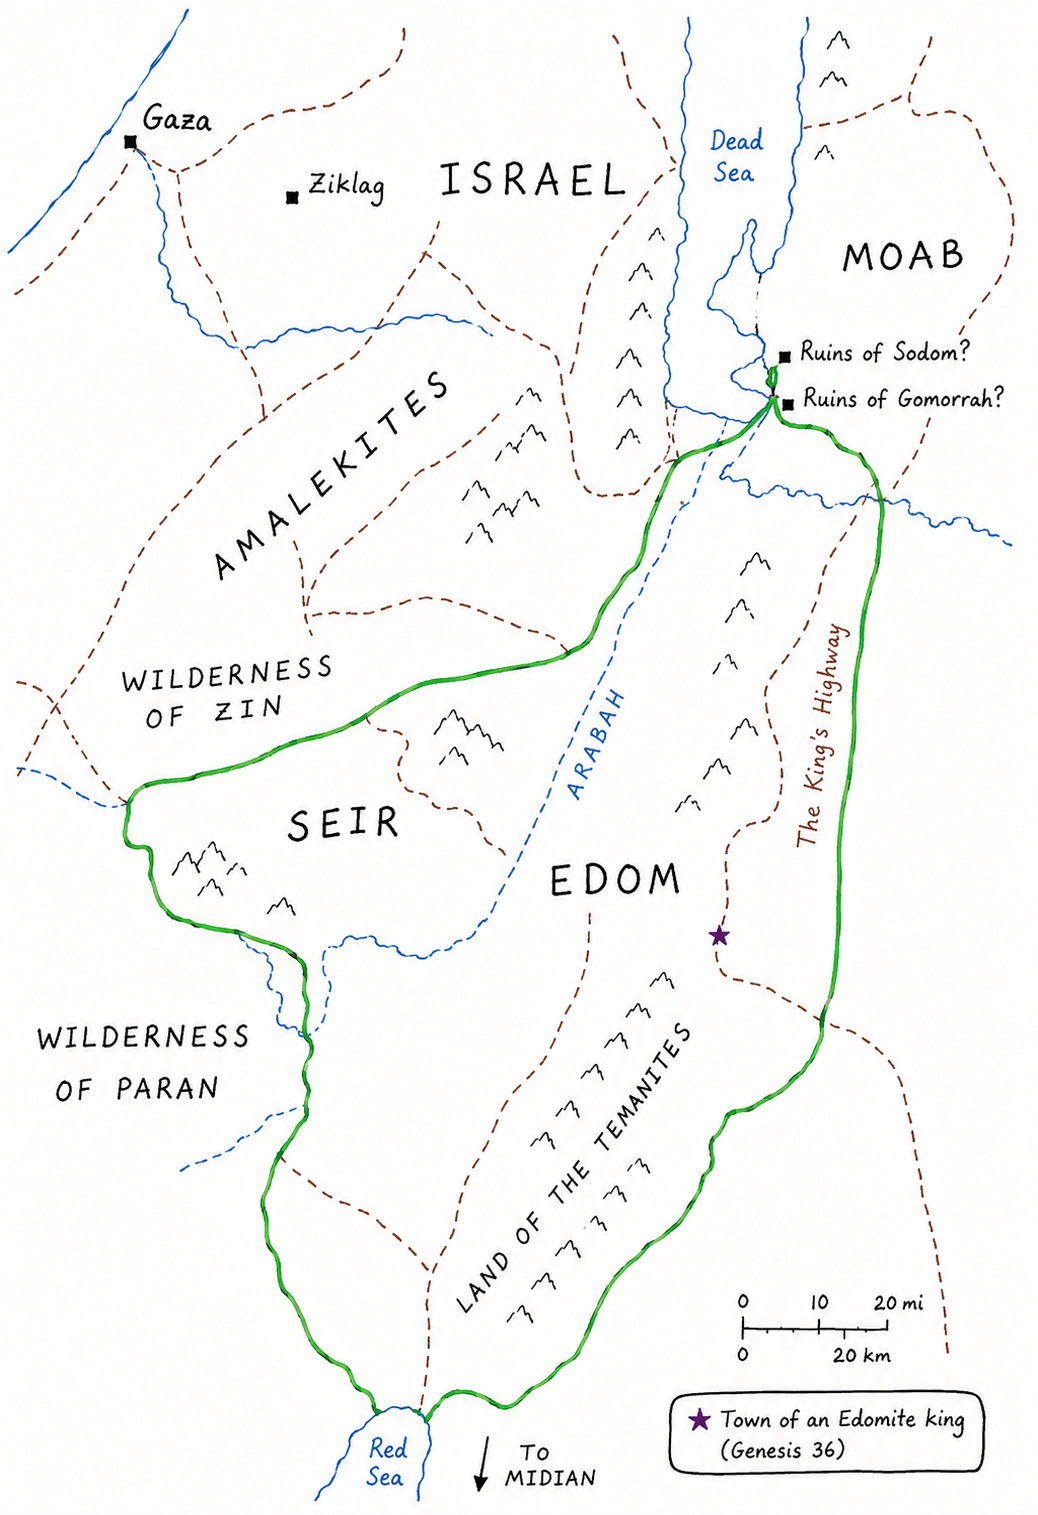
\includegraphics[width=0.9\linewidth]{01-genesis/include/seir.jpg}
	\end{center}

	So Esau is Edom and he comes out all Seir-y.

	Also Edom is \paleo{𐤀𐤃𐤌}.%
	\footnote{They eventually add a \paleo{𐤅} in the middle when matres lectiones catch on.}

	So basically in the era when this section was originally written%
	\footnote{
		A couple thousand years before niqqud get invented.
		Niqqud are the little vowel dots that P really likes.
	} get invented, all three of these words are spelled exactly the same:

	\begin{enumerate}
	\item Edom
	\item Red
	\item Adam (the word for human)
	\end{enumerate}

}

\Verse{26}
{
	\hJ{וְאַחֲרֵי כֵן יָצָא אָחִיו וְיָדוֹ אֹחֶזֶת בַּעֲקֵב עֵשָׂו וַיִּקְרָא שְׁמוֹ יַעֲקֹב וְיִצְחָק בֶּן שִׁשִּׁים שָׁנָה בְּלֶדֶת אֹתָם׃}
}
{
	\eJ{
		And after that his brother came out, and his hand was
		holding Esau’s heel, and he called his name Jacob. And
		Isaac was sixty years old at their birth.
	}
}
{
}

\Verse{27}
{
	\hJ{וַיִּגְדְּלוּ הַנְּעָרִים וַיְהִי עֵשָׂו אִישׁ יֹדֵעַ צַיִד אִישׁ שָׂדֶה וְיַעֲקֹב אִישׁ תָּם יֹשֵׁב אֹהָלִים׃}
}
{
	\eJ{
		And the boys grew up, and Esau was a man who knew hunting,
		a man of the field, and Jacob was a simple man, living in
		tents.
	}
}
{
	Ok so the text notes that:

	\begin{enumerate}
	\item Esau's a man's man, a hunter.
	\item Jacob is more simple and intense.
	\end{enumerate}

	The translation here is a bit strange.

	Most translate (\heb{תם}) as ``simple.''

	The word is from the same root as in Genesis 6:9 when Noah is called ``blameless'' (\heb{תמים}).

	So it's possible that J's saying something more like ``Jacob was an innocent homebody.''

	Which would be particularly ironic\footnote{Aka, very J} given what's about to happen.

	Let's go see.

%	\footnote{
%		Esau. Numerous attempts have been made to denigrate Esau in midrash and
%		even in current biblical interpretation. It is not justified according
%		to the text. The motive is understandable: Jacob’s behavior in the
%		matters of the birthright and the blessing is an embarrassment. Even
%		small children express surprise at what this patriarch does to his
%		brother—and his father. The Torah itself neither denigrates Esau nor
%		justifies Jacob. On the contrary, one of the great qualities of the
%		Tanak is precisely that none of its heroes is perfect. Moreover, Jacob
%		suffers some corresponding recompense for every deception he commits, as
%		do Laban, Rachel, Reuben, Simeon, Levi, Judah, and Joseph’s other
%		brothers. (See the relevant comments below.) The lesson, therefore, is
%		not only that people are not perfect, but also that acts of deception
%		can fester in a family, and that they have consequences. Those who try
%		to excuse Jacob and turn Esau into a villain are unfortunately hiding
%		these essential lessons of the Torah.
%	}
}

\Verse{28}
{
	\hJ{וַיֶּאֱהַב יִצְחָק אֶת עֵשָׂו כִּי צַיִד בְּפִיו וְרִבְקָה אֹהֶבֶת אֶת יַעֲקֹב׃}
}
{
	\eJ{
		And Isaac loved Esau because he put game meat in his
		mouth, and Rebekah loved Jacob.
	}
}
{
	Isaac loved Esau.

	Because reasons.

	Rebecca loved Jacob.

	End of verse.
}

\Verse{29}
{
	\hJ{וַיָּזֶד יַעֲקֹב נָזִיד וַיָּבֹא עֵשָׂו מִן הַשָּׂדֶה וְהוּא עָיֵף׃}
}
{
	\eJ{
		And Jacob made a stew, and Esau came from the field, and
		he was exhausted.
	}
}
{
	Jacob makes some chili or something.

	Esau comes home from hunting.

	Hunting's a more high variance activity than making soup, so apparently he didn't catch anything today.

	\aB{
		Ok so:
	
		1. The stew is Red.
	
		2. The word for Red is ADM (\heb{אדם}).
	
		3. It's the same as the word for Human (i.e., Adam)
	
		4. It's also the same word as Edom.
	
		Make a note of that.
	
		It'll be useful about one sentence from now.
	}
}

\Verse{30}
{
	\hJ{וַיֹּאמֶר עֵשָׂו אֶל יַעֲקֹב הַלְעִיטֵנִי נָא מִן הָאָדֹם הָאָדֹם הַזֶּה כִּי עָיֵף אָנֹכִי עַל כֵּן קָרָא שְׁמוֹ אֱדוֹם׃}
}
{
	\eJ{
		And Esau said to Jacob, “Will you feed me some of the red
		stuff, this red stuff, because I’m exhausted.” (On account
		of this he called his name “Edom.”)
	}
}
{
	So Esau's like:

	\begin{quote}
	Gimmie.

	Please.

	Some.

	The Red.

	The Red.

	This.
	\end{quote}

	That's why we call him Red.

	\begingroup
	\scriptsize
	\setlength{\tabcolsep}{0.35em}
	\Table{|p{0.17\linewidth}|p{0.23\linewidth}|p{0.50\linewidth}|}{
		\hline
		\textbf{Hebrew} & \textbf{Transliteration} & \textbf{Meaning} \\
		\hline
		\heb{ויאמר} & wayyomer & and said \\
		\hline
		\heb{עשו} & ʿEsaw & Esau \\
		\hline
		\heb{אל} & ʾel & to \\
		\hline
		\heb{יעקב} & Yaʿaqov & Jacob \\
		\hline
		\heb{הלעיטני} & halʿiteni & let me gulp down / feed me \\
		\hline
		\heb{נא} & naʾ & please / now \\
		\hline
		\heb{מן} & min & from / some of \\
		\hline
		\heb{האדם} & haʾadom & the red \\
		\hline
		\heb{האדם} & haʾadom & the red \\
		\hline
		\heb{הזה} & hazzeh & this \\
		\hline
		\heb{כי} & ki & because / for \\
		\hline
		\heb{עיף} & ʿayef & exhausted / faint \\
		\hline
		\heb{אנכי} & ʾanokhi & I \\
		\hline
		\heb{על} & ʿal & therefore / on account of \\
		\hline
		\heb{כן} & ken & this / so \\
		\hline
		\heb{קרא} & qaraʾ & was called \\
		\hline
		\heb{שמו} & shemo & his name \\
		\hline
		\heb{אדום} & ʾEdom & Edom \\
		\hline
	}
	\endgroup
}

\Verse{31}
{
	\hJ{וַיֹּאמֶר יַעֲקֹב מִכְרָה כַיּוֹם אֶת בְּכֹרָתְךָ לִי׃}
}
{
	\eJ{And Jacob said, “Sell your birthright to me, today.”}
}
{
	So the Usurper says to the Red Man:

	Give me your birthright and I'll give you the soup.
}

\Verse{32}
{
	\hJ{וַיֹּאמֶר עֵשָׂו הִנֵּה אָנֹכִי הוֹלֵךְ לָמוּת וְלָמָּה זֶּה לִי בְּכֹרָה׃}
}
{
	\eJ{
		And Esau said, “Here I’m going to die, and what use is
		this, that I have a birthright?”
	}
}
{
	And the Red man is like ``No use have birthright if dead. Deal.''
}

\Verse{33}
{
	\hJ{וַיֹּאמֶר יַעֲקֹב הִשָּׁבְעָה לִּי כַּיּוֹם וַיִּשָּׁבַע לוֹ וַיִּמְכֹּר אֶת בְּכֹרָתוֹ לְיַעֲקֹב׃}
}
{
	\eJ{
		And Jacob said, “Swear to me, today.” And he swore to him
		and sold his birthright to Jacob.
	}
}
{
	Jacob makes him swear on it.

	Presumably verbal contracts are binding in ancient Israel.%
	\footnote{Or whatever it was called before the wrestling scene we haven't reached yet.}
}

\Verse{34}
{
	\hJ{וְיַעֲקֹב נָתַן לְעֵשָׂו לֶחֶם וּנְזִיד עֲדָשִׁים וַיֹּאכַל וַיֵּשְׁתְּ וַיָּקם וַיֵּלַךְ וַיִּבֶז עֵשָׂו אֶת הַבְּכֹרָה׃}
}
{
	\eJ{And Jacob gave bread and lentil stew to Esau.
		And he ate and drank and got up and went.
		And Esau disdained the birthright.}
}
{
	So that's how the-guy-who-we'll-eventually-learn-the-nation-is-named-after
	outwitted the Red Man and bought \sout{Manhattan} his birthright real cheap.
}
